\documentclass{article}

\title{Report}
\date{28th October 2018}
\author{Siddharth Nayak EE16B073 }
\usepackage{graphicx}
\usepackage{hyperref}
\usepackage{amsmath}
\usepackage{amsfonts}
\usepackage{amssymb}
\usepackage{float}
\usepackage{geometry}
\geometry{legalpaper, portrait, margin=1in}
\newcommand\tab[1][1cm]{\hspace*{#1}}
\newcommand \Mycomb[2][^n]{\prescript{#1\mkern-0.5mu}{}C_{#2}}

 \hypersetup{
    colorlinks=true,
    linkcolor=blue,
    filecolor=magenta,      
    urlcolor=blue,
}
 
\urlstyle{same}
 
\begin{document}

\maketitle
\newcommand{\norm}[1]{\left\lVert#1\right\rVert}
\pagenumbering{arabic}


\section{Dataset Details}
The MNIST(Modified National Institute of Standards and Technology) dataset contains images of handwritten digits from 0-9. It has 60,000 images for training and 10,000 images for testing.The images are 28x28 pixels grayscale images.Thus the images have only one channel of intensity of the pixels.\\ Note:In this assignment I have used 10,000 images for training.

\section{Visualisation of the Weights}
\begin{figure}[H]
\subfigure{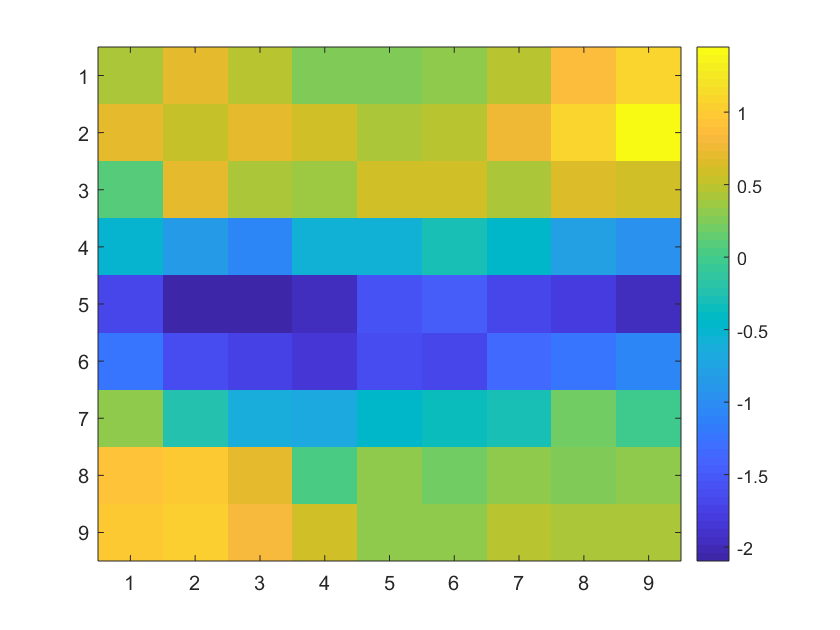
\includegraphics[width=0.45\textwidth]{filter1_weights.png}}
\hspace{0.05\textwidth}
\subfigure{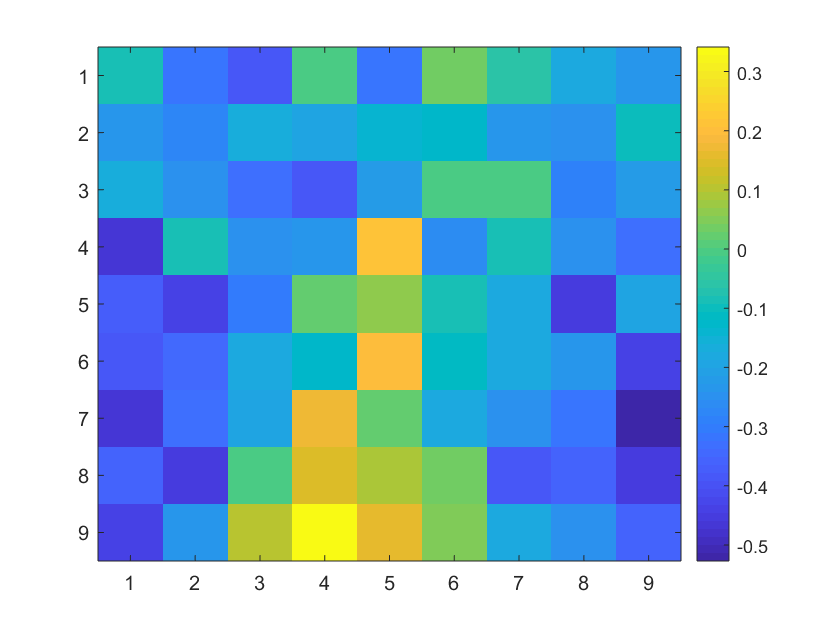
\includegraphics[width=0.45\textwidth]{filter2_weights.png}}
\end{figure}

\begin{figure}[H]
\subfigure{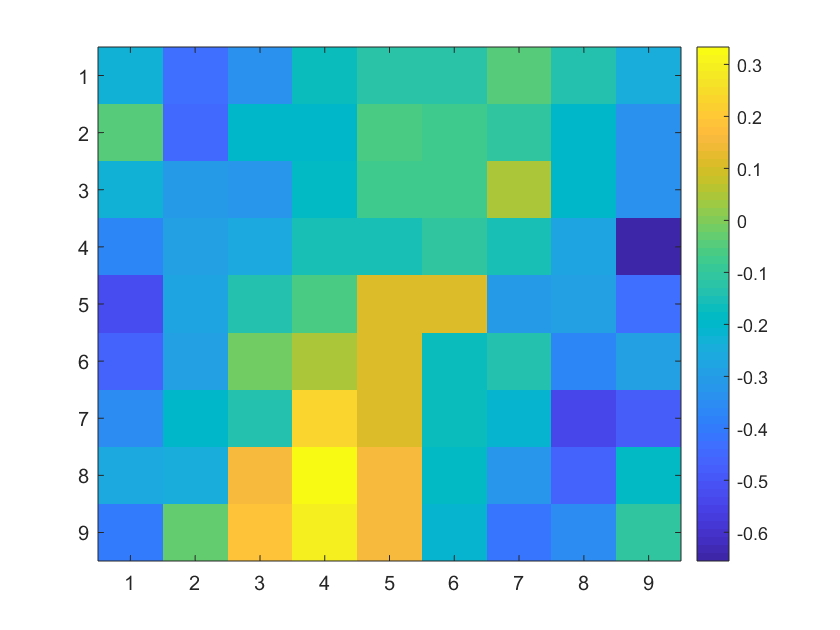
\includegraphics[width=0.45\textwidth]{filter3_weights.png}}
\hspace{0.05\textwidth}
\subfigure{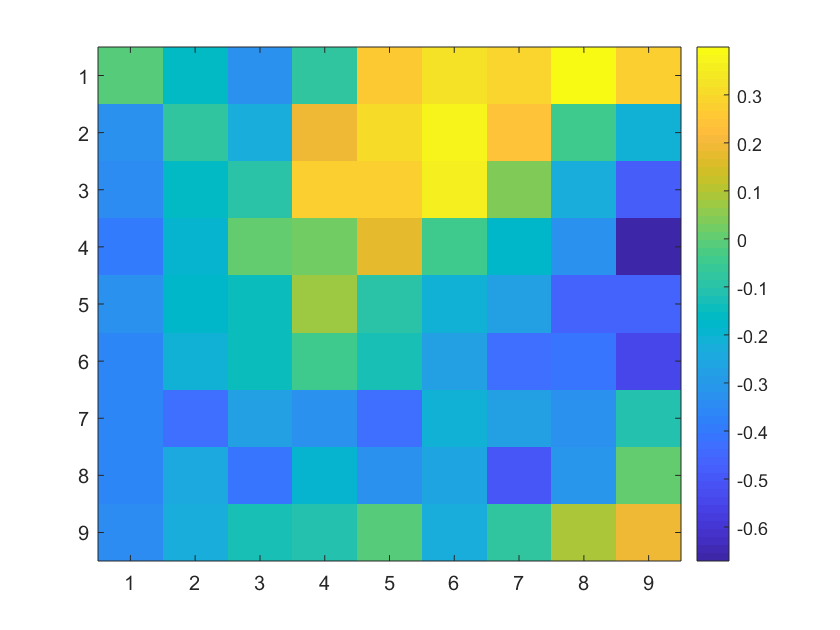
\includegraphics[width=0.45\textwidth]{filter20_weights.png}}
\end{figure}

\begin{figure}[H]
\subfigure{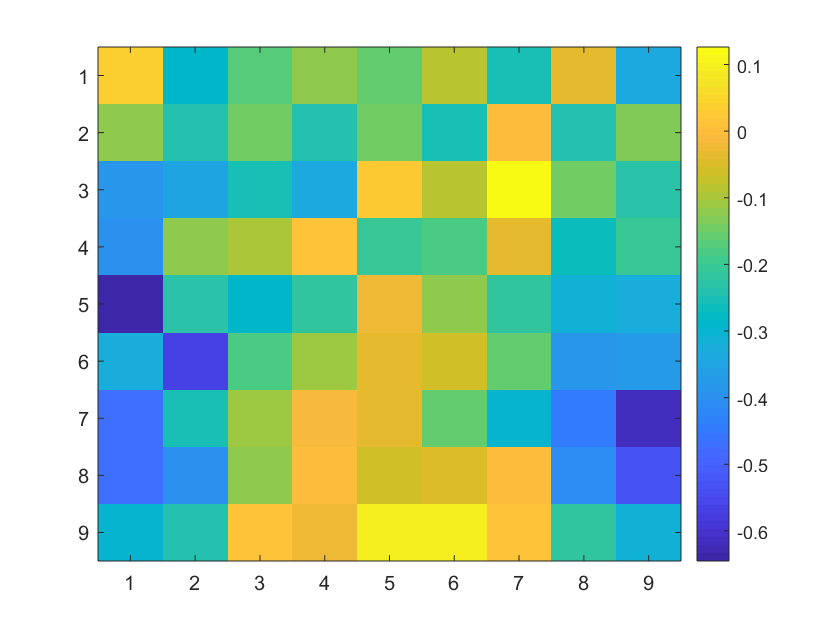
\includegraphics[width=0.45\textwidth]{filter5_weights.png}}
\hspace{0.05\textwidth}
\subfigure{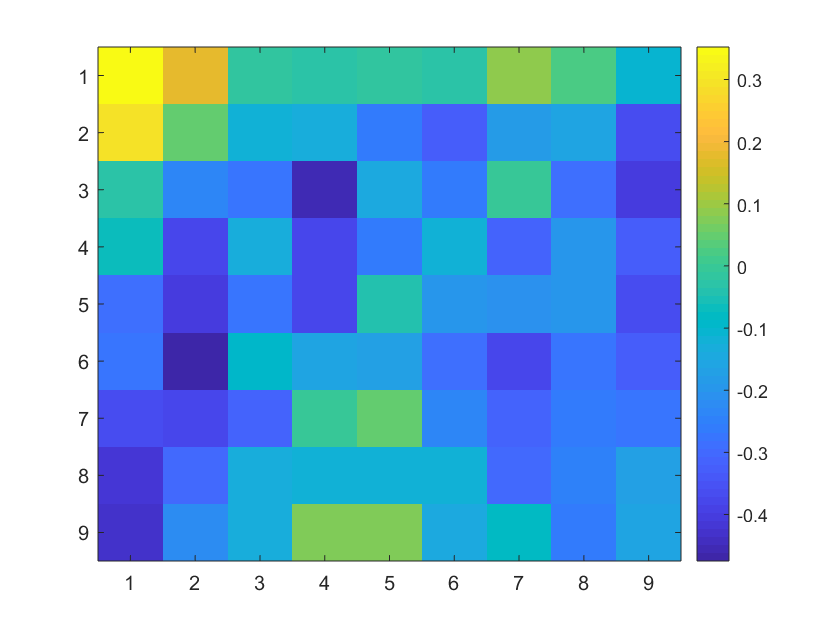
\includegraphics[width=0.45\textwidth]{filter6_weights.png}}
\end{figure}

\begin{figure}[H]
\subfigure{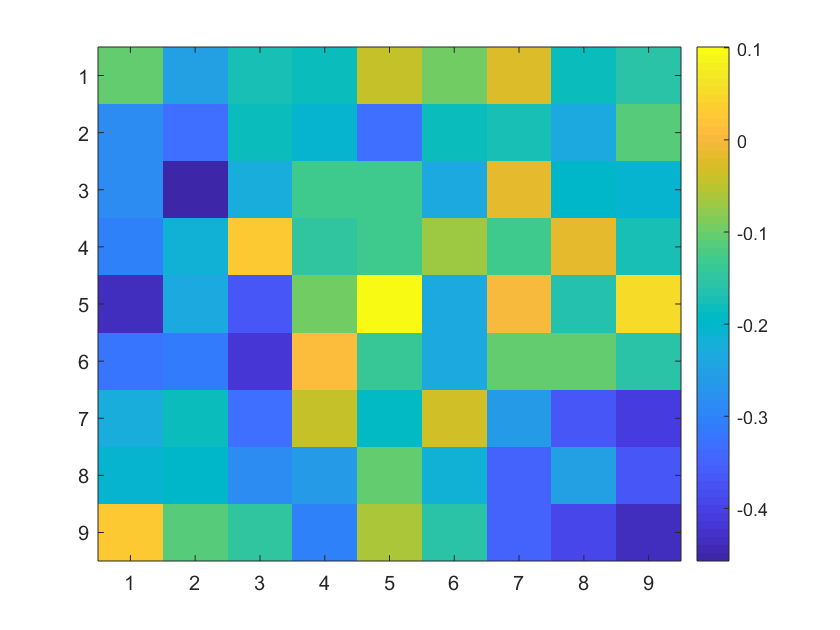
\includegraphics[width=0.45\textwidth]{filter7_weights.png}}
\hspace{0.05\textwidth}
\subfigure{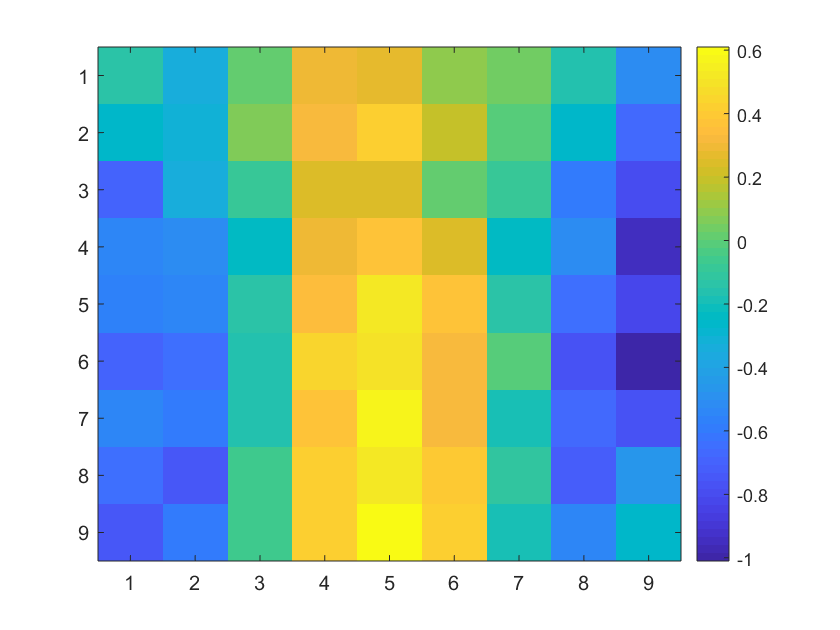
\includegraphics[width=0.45\textwidth]{filter8_weights.png}}
\end{figure}

\begin{figure}[H]
\subfigure{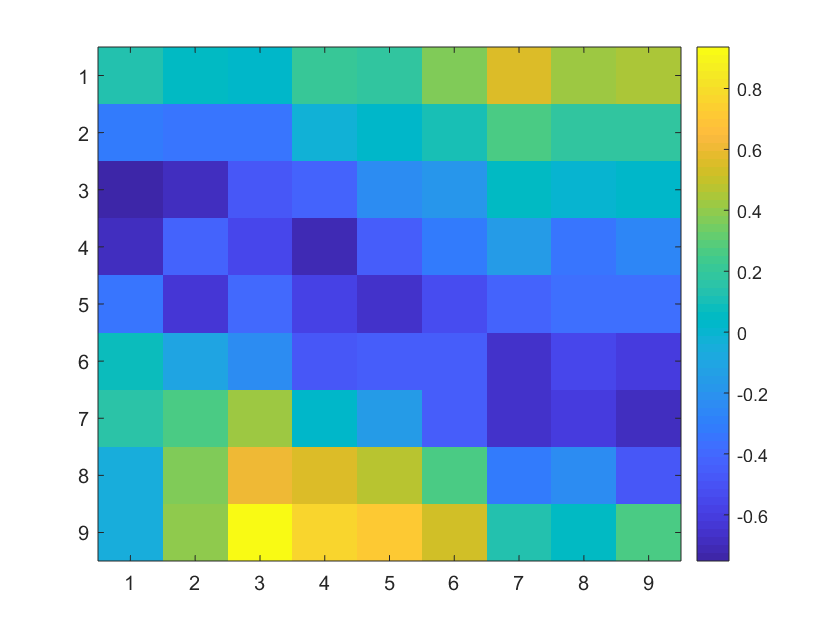
\includegraphics[width=0.45\textwidth]{filter9_weights.png}}
\hspace{0.05\textwidth}
\subfigure{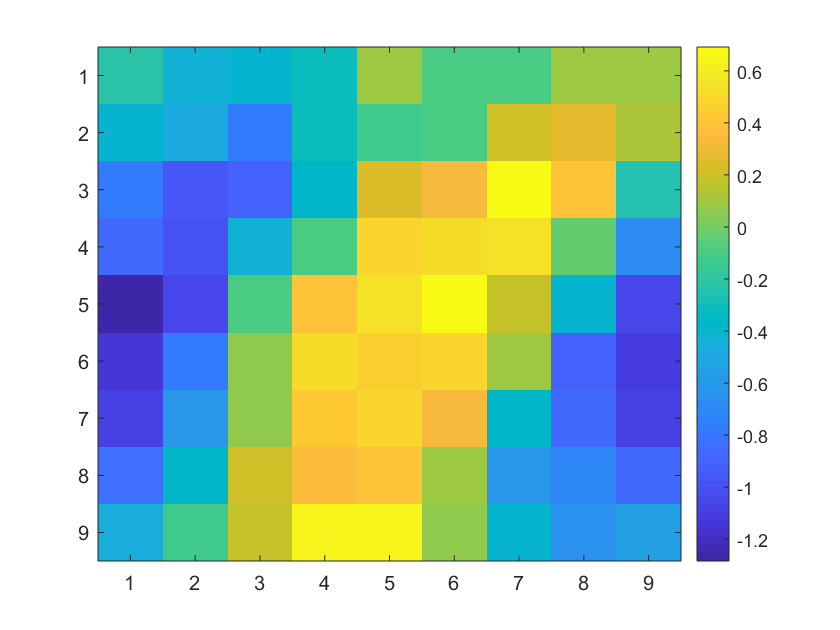
\includegraphics[width=0.45\textwidth]{filter10_weights.png}}
\end{figure}

\begin{figure}[H]
\subfigure{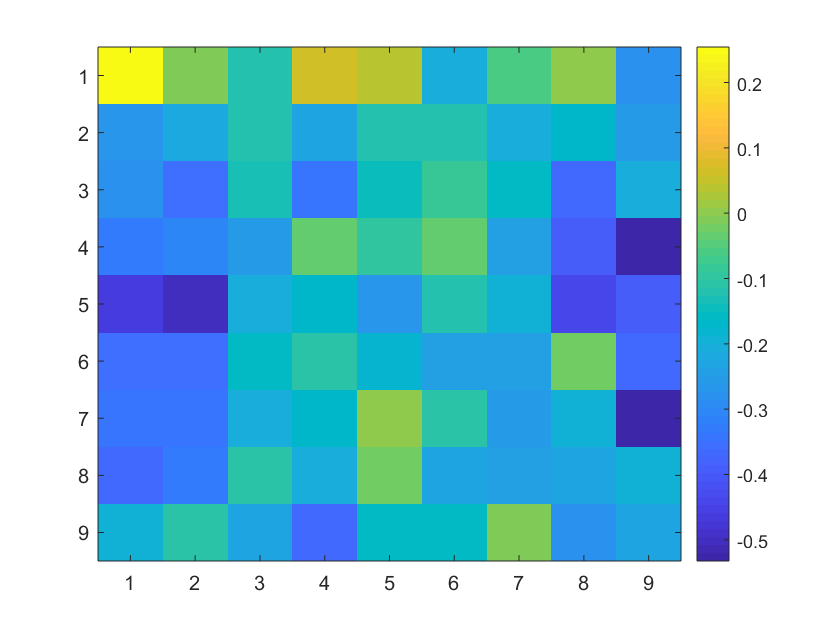
\includegraphics[width=0.45\textwidth]{filter11_weights.png}}
\hspace{0.05\textwidth}
\subfigure{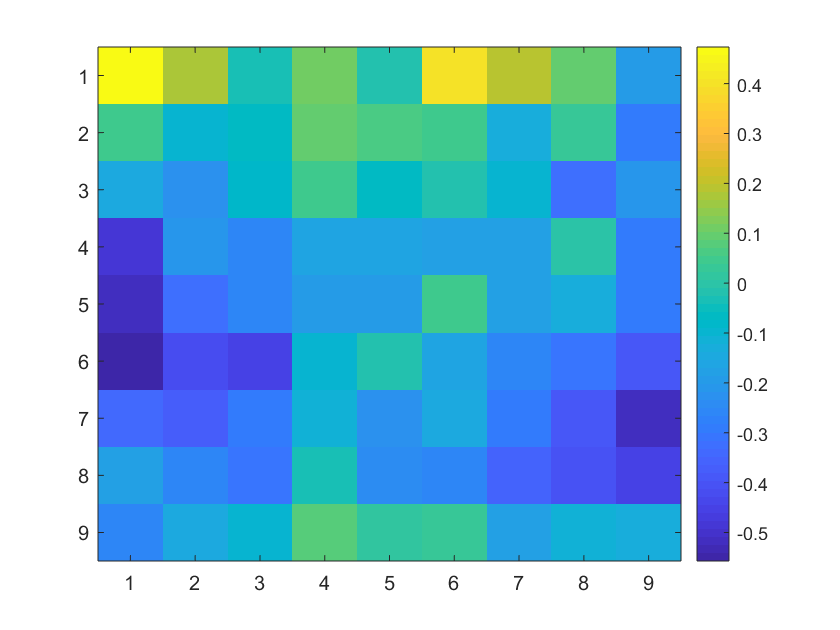
\includegraphics[width=0.45\textwidth]{filter12_weights.png}}
\end{figure}

\begin{figure}[H]
\subfigure{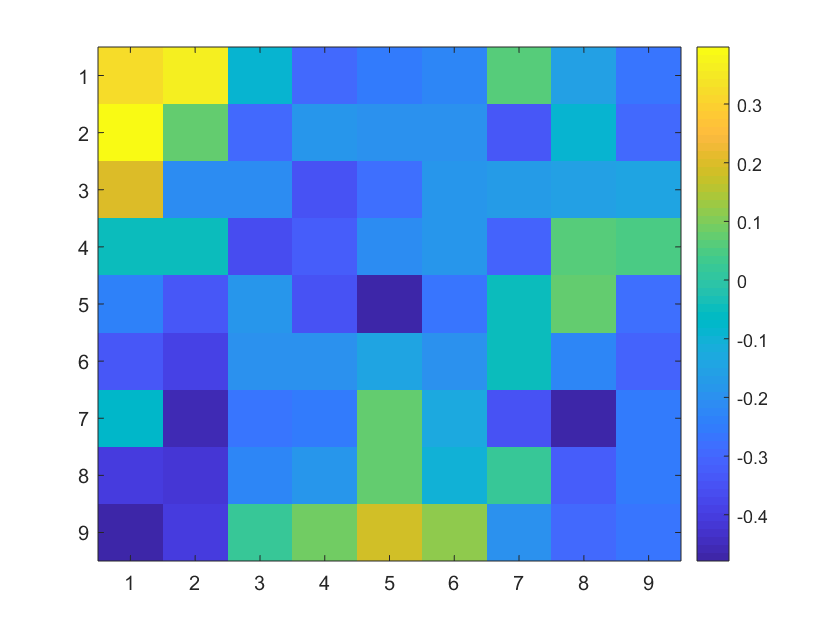
\includegraphics[width=0.45\textwidth]{filter13_weights.png}}
\hspace{0.05\textwidth}
\subfigure{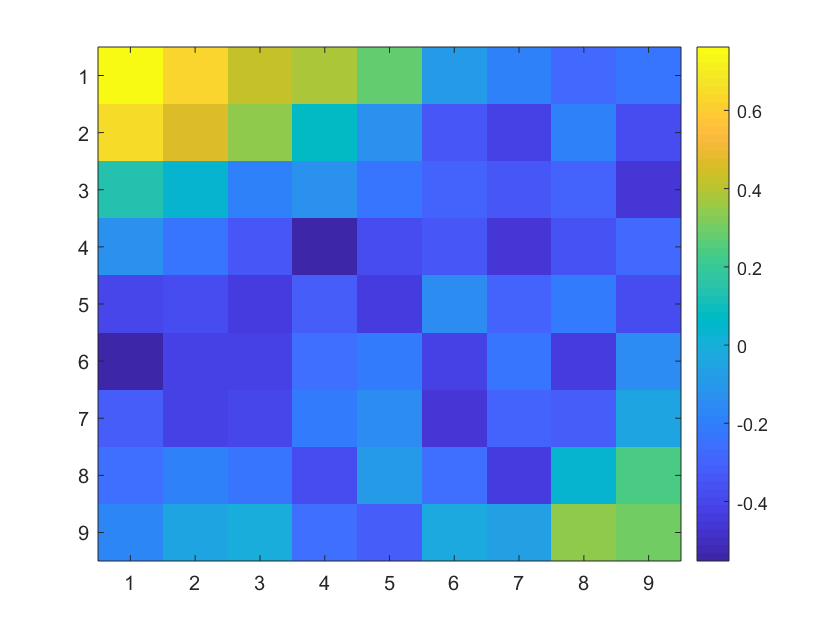
\includegraphics[width=0.45\textwidth]{filter14_weights.png}}
\end{figure}

\begin{figure}[H]
\subfigure{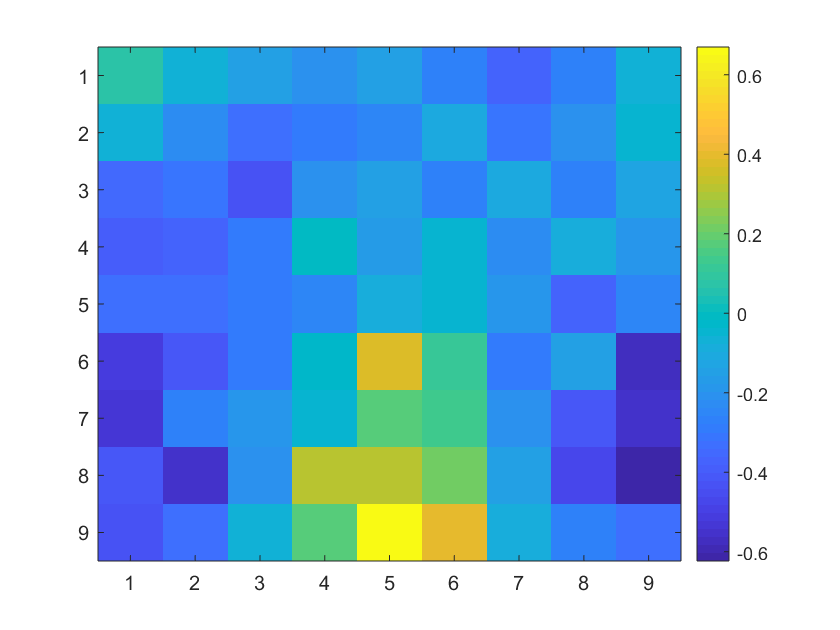
\includegraphics[width=0.45\textwidth]{filter15_weights.png}}
\hspace{0.05\textwidth}
\subfigure{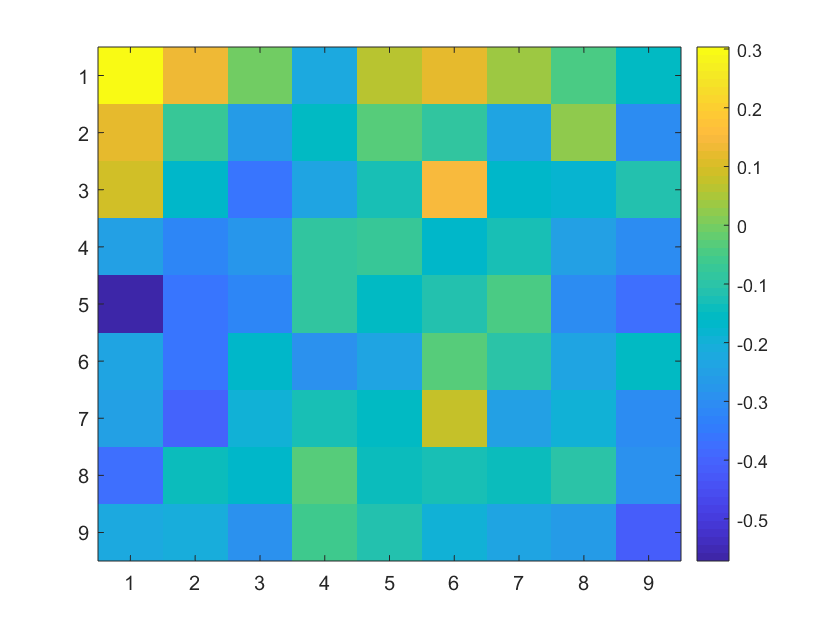
\includegraphics[width=0.45\textwidth]{filter16_weights.png}}
\end{figure}

\begin{figure}[H]
\subfigure{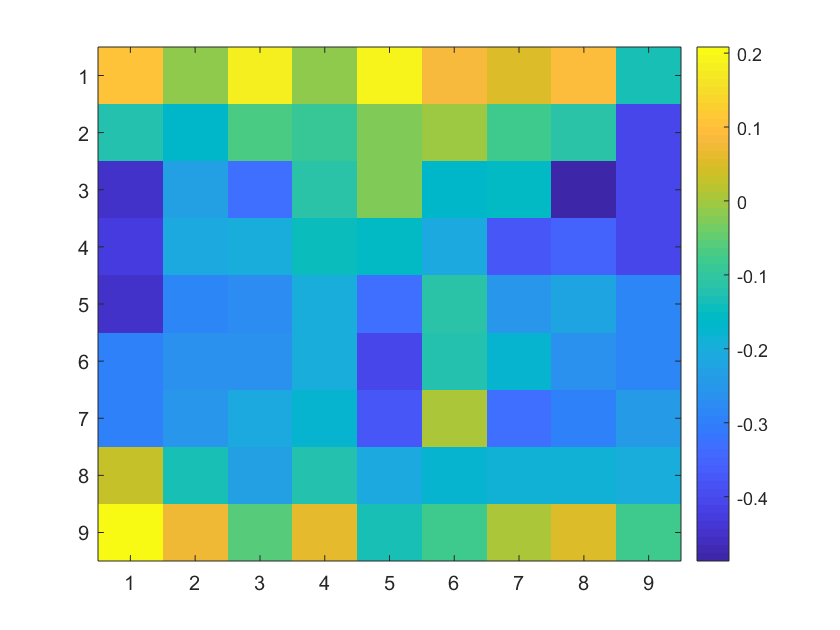
\includegraphics[width=0.45\textwidth]{filter17_weights.png}}
\hspace{0.05\textwidth}
\subfigure{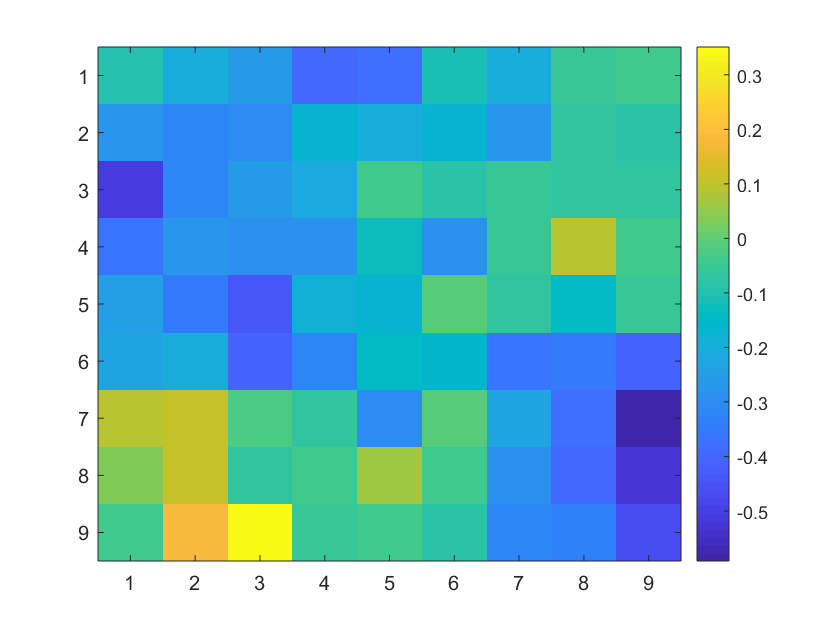
\includegraphics[width=0.45\textwidth]{filter18_weights.png}}
\end{figure}

\begin{figure}[H]
\subfigure{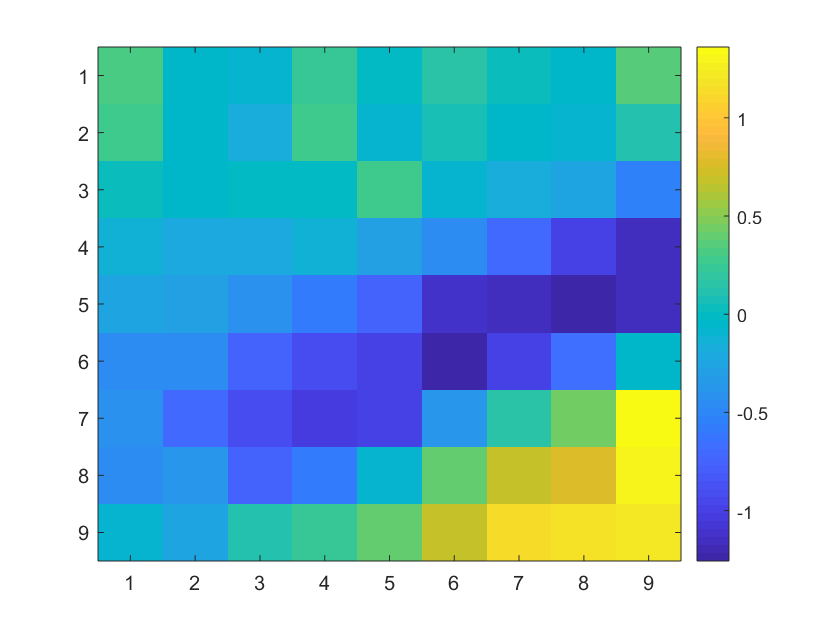
\includegraphics[width=0.45\textwidth]{filter19_weights.png}}
\hspace{0.05\textwidth}
\subfigure{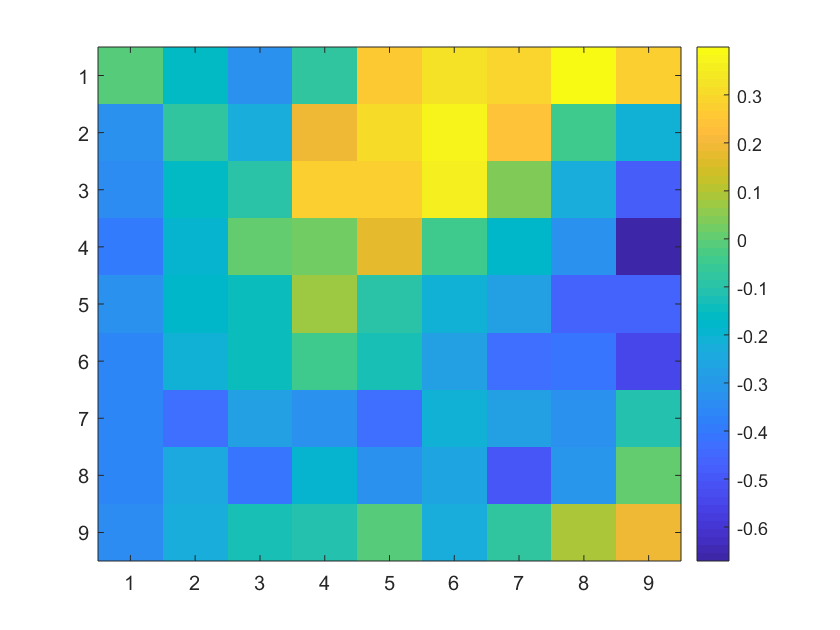
\includegraphics[width=0.45\textwidth]{filter20_weights.png}}
\end{figure}

\section{Activations Visualisation}
\subsection{Image Choosen}
\begin{figure}[H]
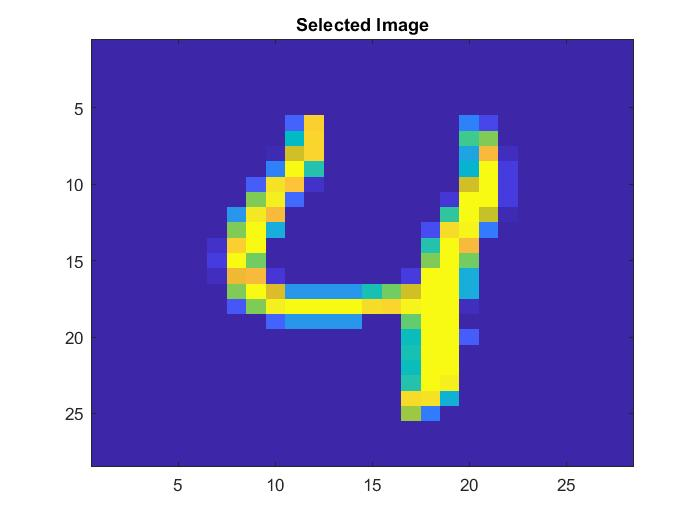
\includegraphics[width=0.65\textwidth]{num.jpg}
\centering
\caption{Image with number 4 in it}
\end{figure}

\subsection{Activations}
\begin{figure}[H]
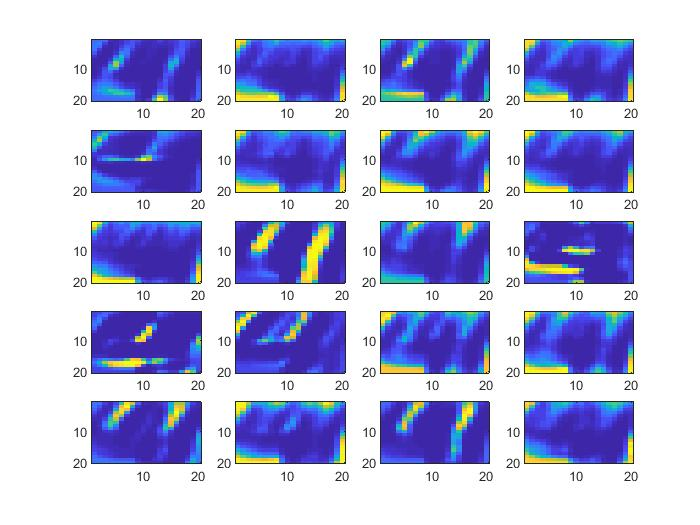
\includegraphics[width=0.65\textwidth]{map.jpg}
\centering
\caption{Activations }
\end{figure}
The activation map in 2nd Column and 3rd Row detects the vertical lines. And the activation map in the 4th Column and 3rd Row detects the horizontal lines.Also the activations hallucinate number 4. i.e we can see the number 4 in the weights. If we input any other number even then we can actually see that number(loosely) in the weights. Thus different weights activate for different numbers and that is how the Convolutional Neural Network distinguishes between different numbers after training.

\section{Changing hyperparameters}
\subsection{Filter Size = 9 and Number of Filters = 20}
\begin{center}
 \begin{tabular}{||c| c| c| c||} 
 \hline
 Number of Epochs & Accuracy (\%)\\ [0.5ex] 
 \hline\hline
 1 & 89.25  \\ 
 \hline
 2 & 92.97 \\ 
 \hline
 3 & 93.4 \\
 \hline
 5 & 93.4  \\
 \hline
 7 & 93.11  \\
 \hline
 9 & 92.2 \\ [1ex] 
 \hline
\end{tabular}
\end{center}

\subsection{Filter Size = 9 and Number of Epochs = 3}
\begin{center}
 \begin{tabular}{||c| c| c| c||} 
 \hline
Number of Filters & Accuracy (\%)\\ [0.5ex] 
 \hline\hline
 10 & 93.57  \\ 
 \hline
 15 & 94.04 \\ 
 \hline
 20 & 93.4 \\
 \hline
 25 & 92.62 \\
 \hline
 
\end{tabular}
\end{center}

\subsection{Number of Filters = 20 and Number of Epochs = 3}
\begin{center}
 \begin{tabular}{||c| c| c| c||} 
 \hline
Filter Size & Accuracy (\%)\\ [0.5ex] 
 \hline\hline
 7 & 93.29  \\ 
 \hline
 9 & 95.4 \\ 
 \hline
 15 & 95.79 \\ 
 \hline
 25 & 96.19 \\
 \hline
 
\end{tabular}
\end{center}

%%%%%%%%%%%%%%%%%%%%%%%%%%%%%%%%%%%%%%%%%%%%%%%%%%%%%%%%%%%%%%%%%%%%%%%%%%%%%%%%%%%%%%%%%%%%%%%%%%%%%%%%%%%%%%%%%%%%%%
\end{document}
